\pagestyle{fancy}
\renewcommand{\theUnit}{4}
\ifthenelse{\isundefined{\UnitPageNumbers}}{}{\setcounter{page}{1}}
\rhead{Chapter \theUnit: Sampling Distributions}
\lhead{Math 3382: Statistical Theory}
%\lhead{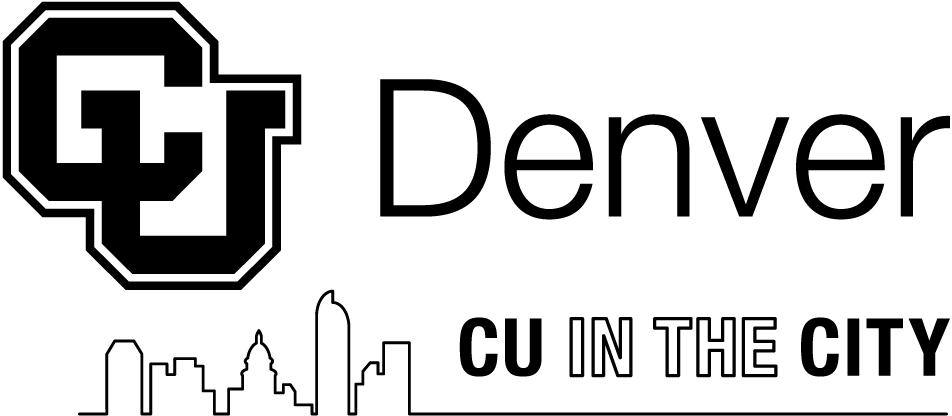
\includegraphics[width=1.25cm]{CUDenver-Logo.png}}
\rfoot{\mypage}
\cfoot{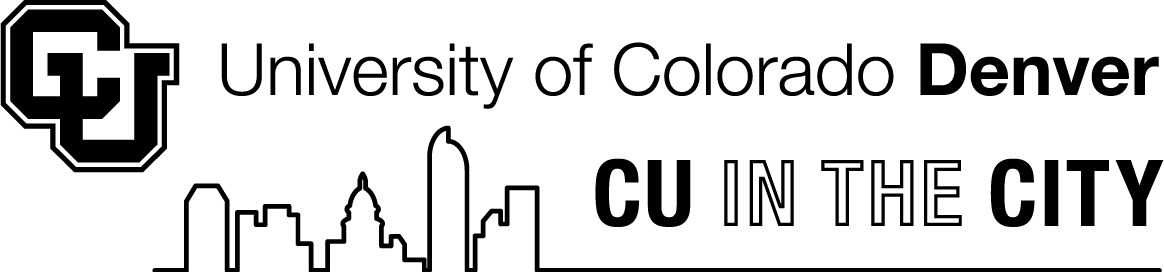
\includegraphics[width=2.25cm]{CUDenver-Logo-coverpage.png}}
\lfoot{Adam Spiegler}
\fancypagestyle{firstfooter}{\footskip = 50pt}
\renewcommand{\footrulewidth}{.4pt}
%%%%%%%%%%%%%%%%%%%%%%%%%%%
\vspace*{-20pt} \thispagestyle{firstfooter}


%\begin{tasks}[counter-format = {(tsk[a])},label-offset = {0.8em},label-format = {\color{black}\bfseries}](2)
\pagebegin{Sampling Distributions}

\bbox
\textbf{\colorb{Statistical inference}} is the process of drawing conclusions about the entire population based on information in a sample.
\bigskip

A \textbf{\colorb{sampling distribution}} is the distribution of sample statistics (such as a mean, proportion, median, maximum, etc.) computed for different samples of the same size from the same population. A sampling distribution shows us how the sample statistic varies from sample to sample.
\ebox

\pagebegin{Sampling from Populations with Different Shapes}

For questions 1-3 below, \textbf{\alert{open the RMarkdown file 09\_Sampling\_Dist.Rmd}} and answer the questions in the RMarkdown file by running R code in that file. Then summarize your answers for each question below.

\bb
\ii Let $X$ denote the distribution of BMI of all adult men. We can approximate this distribution by $X \sim N(26, 4)$. \label{q:bmi}
\[ \bar{x} = \frac{x_1 + x_2 + x_3+x_4}{4}. \]


\begin{center}
\begin{tabular}{|l|c|c|c|c|}
\hline
 \ \ & Population & $n=4$ & $n=9$ & $n=16$ \\
\hline
Shape & Normal & \ \ \ \ \ \ \ \ \ \ \ \ \ \ \ \ \ \ \ \ & \ \ \ \ \ \ \ \ \ \ \ \ \ \ \ \ \ \ \ \ & \ \ \ \ \ \ \ \ \ \ \ \ \ \ \ \ \ \ \ \ \\
\hline
Mean & 26 & & & \\
\hline  
Standard Deviation & 4 & & & \\
\hline  
\end{tabular}
\end{center}

\ii  Let $X$ denote the distribution of the time (in minutes) between successive eruptions (called the wait time) of a certain geyser that is modeled by $X \sim \mbox{Exp} \big( \frac{1}{40} \big)$. \label{q:geyser} %https://www.statology.org/exponential-distribution-real-life-examples/

\begin{center}
\begin{tabular}{|l|c|c|c|c|}
\hline
 \ \ & Population & $n=4$ & $n=9$ & $n=16$ \\
\hline
Shape & Skewed \_\_\_\_\_\_\_\_  & \ \ \ \ \ \ \ \ \ \ \ \ \ \ \ \ \ \ \ \ & \ \ \ \ \ \ \ \ \ \ \ \ \ \ \ \ \ \ \ \ & \ \ \ \ \ \ \ \ \ \ \ \ \ \ \ \ \ \ \ \ \\
\hline
Mean & 40 & & & \\
\hline  
Standard Deviation & $\sqrt{40}$ & & & \\
\hline  
\end{tabular}
\end{center}

\ii The dataset  \colorg{quakes}  in R has the locations of 1000 seismic events that occurred near Fiji since 1964 with body wave magnitude (mb)  $> 4.0$. Assume this data represents the population of all such earthquakes near Fiji since 1964. Let $X$ denote the distribution of the depths (in km) where all such earthquakes occurred. Note this data is approximately \alert{bimodal}. \label{q:quake}

\begin{center}
\begin{tabular}{|l|c|c|c|c|}
\hline
 \ \ & Population & $n=4$ & $n=9$ & $n=16$ \\
\hline
Shape & Bimodal & \ \ \ \ \ \ \ \ \ \ \ \ \ \ \ \ \ \ \ \ & \ \ \ \ \ \ \ \ \ \ \ \ \ \ \ \ \ \ \ \ & \ \ \ \ \ \ \ \ \ \ \ \ \ \ \ \ \ \ \ \ \\
\hline
Mean &  & & & \\
\hline  
Standard Deviation &  & & & \\
\hline  
\end{tabular}
\end{center}

\ee


\clearpage

\pagebegin{Notation}

\bbox
\bi
\ii When describing the \alert{mean} of a distribution we use the notation:
\bi
\ii[$\circ$] Population mean: \alert{$\mu_X$}
\ii[$\circ$] Sample mean:  \alert{$\bar{x}$}
\ii[$\circ$] Center of the Sampling distribution for a mean:  \alert{$\mu_{\overline{X}}$}
\ei
\ii When describing the \alert{standard deviation} of a distribution we use the notation:
\bi
\ii[$\circ$] Population standard deviation:  \alert{$\sigma_X$}
\ii[$\circ$] Sample standard deviation:  \alert{$s_X$}
\ii[$\circ$] Spread of the sampling distribution is called the \alert{Standard Error}.
\bi
\ii[$\diamond$] The standard error measures the variability in sample statistics due to randomness.
\ii[$\diamond$] We use the notation \alert{$\mbox{SE}(\overline{X}) = \sigma_{\overline{X}}$}.
\ei
\ei
\ei
\ebox

\bb[resume]
\ii In each of the three sampling distributions we examined, lets summarize what seems to be happening as the size of the samples, $n$, is increased.

\bb
\ii Does the shape of the sampling distribution stay the same as the population or does it change as $n$ increases? \vfill

\ii Does the center of the sampling distribution, $\mu_{\overline{X}}$, stay the same or change as $n$ increases? How does the value of $\mu_{\overline{X}}$ compare to the population mean $\mu_X$? \vfill

\ii Does the standard error of the sampling distribution, $\mbox{SE}(\overline{X})$, stay the same or change as $n$ increases?  \vfill

\ee
\ee

\clearpage

\pagebegin{Central Limit Theorem for Means}

\bbox
Let $X_1, X_2, \ldots , X_n$ be independent, identically distributed (iid) random variables from a population with mean and
standard deviation $\mu$ and $\sigma$, then as long as $n$ is large enough \colorb{($\mathbf{n \geq 30}$)}, the sampling distribution for the mean, $\bar{X}$ will:
\bi
\ii Be (approximately) normally distribution.
\ii Have mean equal to the mean of the population, $\mu$.
\ii Have standard error $\mbox{SE}(\bar{X}) = \frac{\sigma}{\sqrt{n}}$.
\ei

We summarize the results more concisely below:

\alert{ \[ \overline{X} \sim N \left( \mu_{\overline{X}} , \sigma_{\overline{X}} \right) = N \left( \mu  , \frac{\sigma}{\sqrt{n}} \right) \] }

\ebox

\bb[resume]
\ii Recall the distribution of adult male BMI,  $X \sim N(26,4)$, from question \ref{q:bmi} and answer the questions below.

\bb
\ii What is the probability of randomly select one adult man that has a BMI greater than 28? \vfill

\ii If you construct a sampling distribution for the mean BMI of adult males using random samples each size $n=50$, approximate the shape, center, and standard error of the sampling distribution. \vfill

\ii If you construct a sampling distribution for the mean wait time between geyser eruptions using random samples each size $n=100$, approximate the shape, center, and standard error of the sampling distribution. \vfill

\ii What is the probability of picking a random sample of $n=100$ adult men that has a sample mean BMI greater than 28? \vfill
\ee
\ee

\clearpage

\pagebegin{Independent and Identically Distributed Random Variables}

\bbox
The random variables $X_1, X_2, \ldots , X_n$ are said to be \alert{independent and identically distributed (iid)} if
\bi
\ii The $X_i$'s are independent random variables (the value of $X_i$ does not effect the value of $X_j$ for $i \ne j$).
\ii Every $X_i$ has the same probability distribution.
\ii Such a collection of random variables is called a \alert{simple random sample} of size $n$.
\ei
For example:
\bi
\ii Measure the BMI of $n$ randomly selected adult men.
\ii Measure the weight time of $n$ randomly selected eruptions of a geyser.
\ii Measure the depth of $n$ randomly selected $n$ earthquakes that occurred near Fiji since 1964.
\ei
\ebox

